\documentclass[11pt]{article}
\usepackage[margin=0.6in]{geometry}
\usepackage{amssymb, amsmath, amsfonts, amsthm}
\usepackage{mathpazo}
\usepackage{setspace}
\usepackage{fancyhdr}
\usepackage{enumerate}
\usepackage{tikz}
\usepackage{float}
\usetikzlibrary{automata,positioning}
\usepackage{fancybox, graphicx}

\pagestyle{fancyplain}
\lhead{\textbf{\NAME\ }}
\rhead{CPSC 313, \today}

\newcommand\question[2]{
\shadowbox{
\begin{minipage}{45em}\vspace{1ex}\textbf{Problem #1}
\newline
\vspace{1ex}
\end{minipage}
}
\vspace{1ex}
}

\begin{document}
\linespread{0.9}
\newcommand\NAME{Eddy Qiang}
\question{1}{John X and Jane Y}
\begin{enumerate}

%dfa
\begin{center}
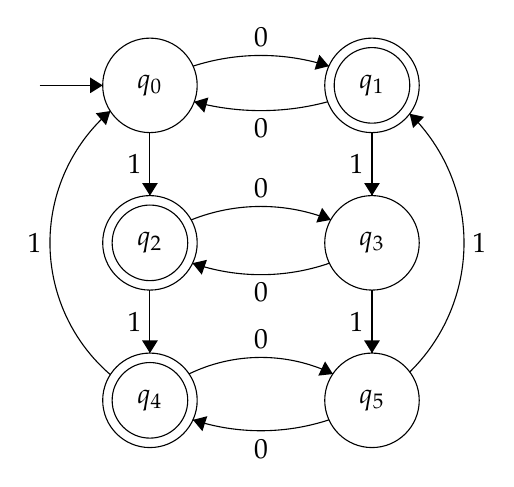
\begin{tikzpicture}[scale=0.2]
\tikzstyle{every node}+=[inner sep=0pt]
\draw [black] (22.2,-15.3) circle (3);
\draw (22.2,-15.3) node {$q_0$};
\draw [black] (36.3,-15.3) circle (3);
\draw (36.3,-15.3) node {$q_1$};
\draw [black] (36.3,-15.3) circle (2.4);
\draw [black] (22.2,-25.3) circle (3);
\draw (22.2,-25.3) node {$q_2$};
\draw [black] (22.2,-25.3) circle (2.4);
\draw [black] (36.3,-25.3) circle (3);
\draw (36.3,-25.3) node {$q_3$};
\draw [black] (22.2,-35.3) circle (3);
\draw (22.2,-35.3) node {$q_4$};
\draw [black] (22.2,-35.3) circle (2.4);
\draw [black] (36.3,-35.3) circle (3);
\draw (36.3,-35.3) node {$q_5$};
\draw [black] (33.491,-16.342) arc (-74.9109:-105.0891:16.293);
\fill [black] (25.01,-16.34) -- (25.65,-17.03) -- (25.91,-16.07);
\draw (29.25,-17.4) node [below] {$0$};
\draw [black] (24.814,-23.845) arc (111.87811:68.12189:11.903);
\fill [black] (33.69,-23.84) -- (33.13,-23.08) -- (32.76,-24.01);
\draw (29.25,-22.49) node [above] {$0$};
\draw [black] (33.599,-26.591) arc (-70.91883:-109.08117:13.303);
\fill [black] (24.9,-26.59) -- (25.49,-27.32) -- (25.82,-26.38);
\draw (29.25,-27.82) node [below] {$0$};
\draw [black] (24.677,-33.625) arc (115.86902:64.13098:10.482);
\fill [black] (33.82,-33.63) -- (33.32,-32.83) -- (32.89,-33.73);
\draw (29.25,-32.07) node [above] {$0$};
\draw [black] (33.574,-36.538) arc (-71.78375:-108.21625:13.832);
\fill [black] (24.93,-36.54) -- (25.53,-37.26) -- (25.84,-36.31);
\draw (29.25,-37.73) node [below] {$0$};
\draw [black] (24.934,-14.08) arc (107.923:72.077:14.024);
\fill [black] (33.57,-14.08) -- (32.96,-13.36) -- (32.65,-14.31);
\draw (29.25,-12.9) node [above] {$0$};
\draw [black] (22.2,-18.3) -- (22.2,-22.3);
\fill [black] (22.2,-22.3) -- (22.7,-21.5) -- (21.7,-21.5);
\draw (21.7,-20.3) node [left] {$1$};
\draw [black] (22.2,-28.3) -- (22.2,-32.3);
\fill [black] (22.2,-32.3) -- (22.7,-31.5) -- (21.7,-31.5);
\draw (21.7,-30.3) node [left] {$1$};
\draw [black] (36.3,-18.3) -- (36.3,-22.3);
\fill [black] (36.3,-22.3) -- (36.8,-21.5) -- (35.8,-21.5);
\draw (35.8,-20.3) node [left] {$1$};
\draw [black] (36.3,-28.3) -- (36.3,-32.3);
\fill [black] (36.3,-32.3) -- (36.8,-31.5) -- (35.8,-31.5);
\draw (35.8,-30.3) node [left] {$1$};
\draw [black] (38.693,-17.096) arc (45.62578:-45.62578:11.478);
\fill [black] (38.69,-17.1) -- (38.91,-18.01) -- (39.61,-17.3);
\draw (42.64,-25.3) node [right] {$1$};
\draw [black] (19.69,-33.673) arc (-130.72919:-229.27081:11.049);
\fill [black] (19.69,-16.93) -- (18.76,-17.07) -- (19.41,-17.83);
\draw (15.35,-25.3) node [left] {$1$};
\draw [black] (15.2,-15.3) -- (19.2,-15.3);
\fill [black] (19.2,-15.3) -- (18.4,-14.8) -- (18.4,-15.8);
\end{tikzpicture}
\end{center}

%explanation
My DFA is the cross product of a DFA that accepts the number of 0's that is even, and a DFA that accepts the number of 1's that is not divisible by 3. 
\newline

q\textsubscript{1}, q\textsubscript{2}, q\textsubscript{4} are the accept states because the condition 'if and only if' is only true when the antecedent and consequent are both true, or both false. Therefore q\textsubscript{2} and q\textsubscript{4} are accept states because the number of 0's is even and the number of 1's is not divisible by 3. And q\textsubscript{1} is an accept state because the number of 0's is odd and the number of 1's is divisible by 3. Therefore my DFA is correct as it will accept the language all strings in which the number of 0's is even if and only if the number of 1's is
not divisible by 3.

\end{enumerate}
\newpage

\question{2}{John X and Jane Y} % add your collaborators here.

% begin your solution here
\begin{enumerate}

%dfa
\begin{center}
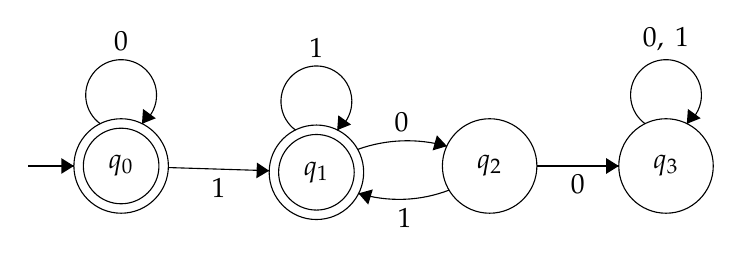
\begin{tikzpicture}[scale=0.2]
\tikzstyle{every node}+=[inner sep=0pt]
\draw [black] (20.7,-29.8) circle (3);
\draw (20.7,-29.8) node {$q_0$};
\draw [black] (20.7,-29.8) circle (2.4);
\draw [black] (33.1,-30.2) circle (3);
\draw (33.1,-30.2) node {$q_1$};
\draw [black] (33.1,-30.2) circle (2.4);
\draw [black] (44.1,-29.8) circle (3);
\draw (44.1,-29.8) node {$q_2$};
\draw [black] (55.3,-29.8) circle (3);
\draw (55.3,-29.8) node {$q_3$};
\draw [black] (19.377,-27.12) arc (234:-54:2.25);
\draw (20.7,-22.55) node [above] {$0$};
\fill [black] (22.02,-27.12) -- (22.9,-26.77) -- (22.09,-26.18);
\draw [black] (23.7,-29.9) -- (30.1,-30.1);
\fill [black] (30.1,-30.1) -- (29.32,-29.58) -- (29.29,-30.58);
\draw (26.88,-30.53) node [below] {$1$};
\draw [black] (31.777,-27.52) arc (234:-54:2.25);
\draw (33.1,-22.95) node [above] {$1$};
\fill [black] (34.42,-27.52) -- (35.3,-27.17) -- (34.49,-26.58);
\draw [black] (35.711,-28.75) arc (109.82474:74.34039:9.323);
\fill [black] (41.39,-28.54) -- (40.75,-27.85) -- (40.48,-28.81);
\draw (38.51,-27.67) node [above] {$0$};
\draw [black] (41.535,-31.328) arc (-68.9117:-106.92317:8.859);
\fill [black] (35.77,-31.54) -- (36.39,-32.25) -- (36.68,-31.29);
\draw (38.7,-32.45) node [below] {$1$};
\draw [black] (47.1,-29.8) -- (52.3,-29.8);
\fill [black] (52.3,-29.8) -- (51.5,-29.3) -- (51.5,-30.3);
\draw (49.7,-30.3) node [below] {$0$};
\draw [black] (53.977,-27.12) arc (234:-54:2.25);
\draw (55.3,-22.55) node [above] {$0,\mbox{ }1$};
\fill [black] (56.62,-27.12) -- (57.5,-26.77) -- (56.69,-26.18);
\draw [black] (14.8,-29.8) -- (17.7,-29.8);
\fill [black] (17.7,-29.8) -- (16.9,-29.3) -- (16.9,-30.3);
\end{tikzpicture}
\end{center}

%explanation
The DFA I have constructed will accept the language because any number of leading 0's in the string will be accepted in q\textsubscript{0}. Then if any number of 1's follow it will be accepted in q\textsubscript{1}. q\textsubscript{2} and q\textsubscript{3} are designed to reject strings not in this language. It does so by making sure there is always a 1 after a 0, and also if there is not a second 0 after a 1. 


\end{enumerate}
\newpage

\question{3}{John X and Jane Y} % add your collaborators here.

% begin your solution here
\begin{enumerate}

%nfa
\begin{center}
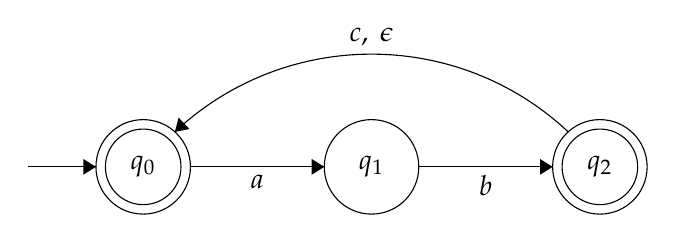
\begin{tikzpicture}[scale=0.2]
\tikzstyle{every node}+=[inner sep=0pt]
\draw [black] (29.6,-30.4) circle (3);
\draw (29.6,-30.4) node {$q_0$};
\draw [black] (29.6,-30.4) circle (2.4);
\draw [black] (44.1,-30.4) circle (3);
\draw (44.1,-30.4) node {$q_1$};
\draw [black] (58.6,-30.4) circle (3);
\draw (58.6,-30.4) node {$q_2$};
\draw [black] (58.6,-30.4) circle (2.4);
\draw [black] (32.6,-30.4) -- (41.1,-30.4);
\fill [black] (41.1,-30.4) -- (40.3,-29.9) -- (40.3,-30.9);
\draw (36.85,-30.9) node [below] {$a$};
\draw [black] (47.1,-30.4) -- (55.6,-30.4);
\fill [black] (55.6,-30.4) -- (54.8,-29.9) -- (54.8,-30.9);
\draw (51.35,-30.9) node [below] {$b$};
\draw [black] (31.611,-28.179) arc (133.13845:46.86155:18.265);
\fill [black] (31.61,-28.18) -- (32.54,-28) -- (31.85,-27.27);
\draw (44.1,-22.74) node [above] {$c,\mbox{ }\epsilon$};
\draw [black] (22.3,-30.4) -- (26.6,-30.4);
\fill [black] (26.6,-30.4) -- (25.8,-29.9) -- (25.8,-30.9);
\end{tikzpicture}
\end{center}

%explanation
My NFA construction has three 3 states. The NFA checks for if there is a 'ab', then it will start a new thread, accepting anything that follows that is not a 'b', thus it will reject strings like abb. If it sees a 'a' after 'ab' the new thread will effectively allow it to go into q\textsubscript{1} which starts the cycle again. Therefore this NFA can accept any combination of 'ab' and 'abc' while rejecting those strings that are not a part of this language.

\end{enumerate}
\newpage

\question{4}{John X and Jane Y} % add your collaborators here.

% begin your solution here
\begin{enumerate}
\item Here is the solution for part 1.

L\textsubscript{2} will accept strings where the difference of the number of a's and b's is no greater than 2. So when you concatenate L\textsubscript{b} with it, the new language will contain at least 4 b's. The intersection between this and L\textsubscript{2} will have to contain the strings with at least 4 b's, so then there must be so there must be at least 2 a's as well to be a part of L\textsubscript{2}. Then lastly it is concatenated with L\textsubscript{a} which adds two more a's to it so now it will have at least four a's with a equal number of b's.
{

L = L\textsubscript{a}(L\textsubscript{2}L\textsubscript{b} \cap L\textsubscript{2}) = \{a\textsuperscript{i}b\textsuperscript{j} \  \vert \ i \geq 4 \ , \ j=i\}
\newline
}

\item Here is the solution for part 2.
\newline
This NFA will recognize strings that contain two 0's separated by a sub-string with a length that is a multiple of 3. The regular expression for this language is (0+1)*0((0+1)(0+1)(0+1))*0(0+1)*. 
\newline
\newline
The expression is correct because the expression starts and ends with (0+1)*0...*0(0+1)*, this part will require there be at least two 0's. The inside part ((0+1)(0+1)(0+1))* will require you to choose either a 0 or 1 three times, and since it is closed under *, the length can be any multiple of 3. Therefore this expression will recognize strings that contain two 0's separated by a sub-string with a length that is a multiple of 3.
\end{enumerate}
\newpage
\end{document}